\documentclass{standalone}
\usepackage{tikz}
\usetikzlibrary{patterns, positioning}

\begin{document}
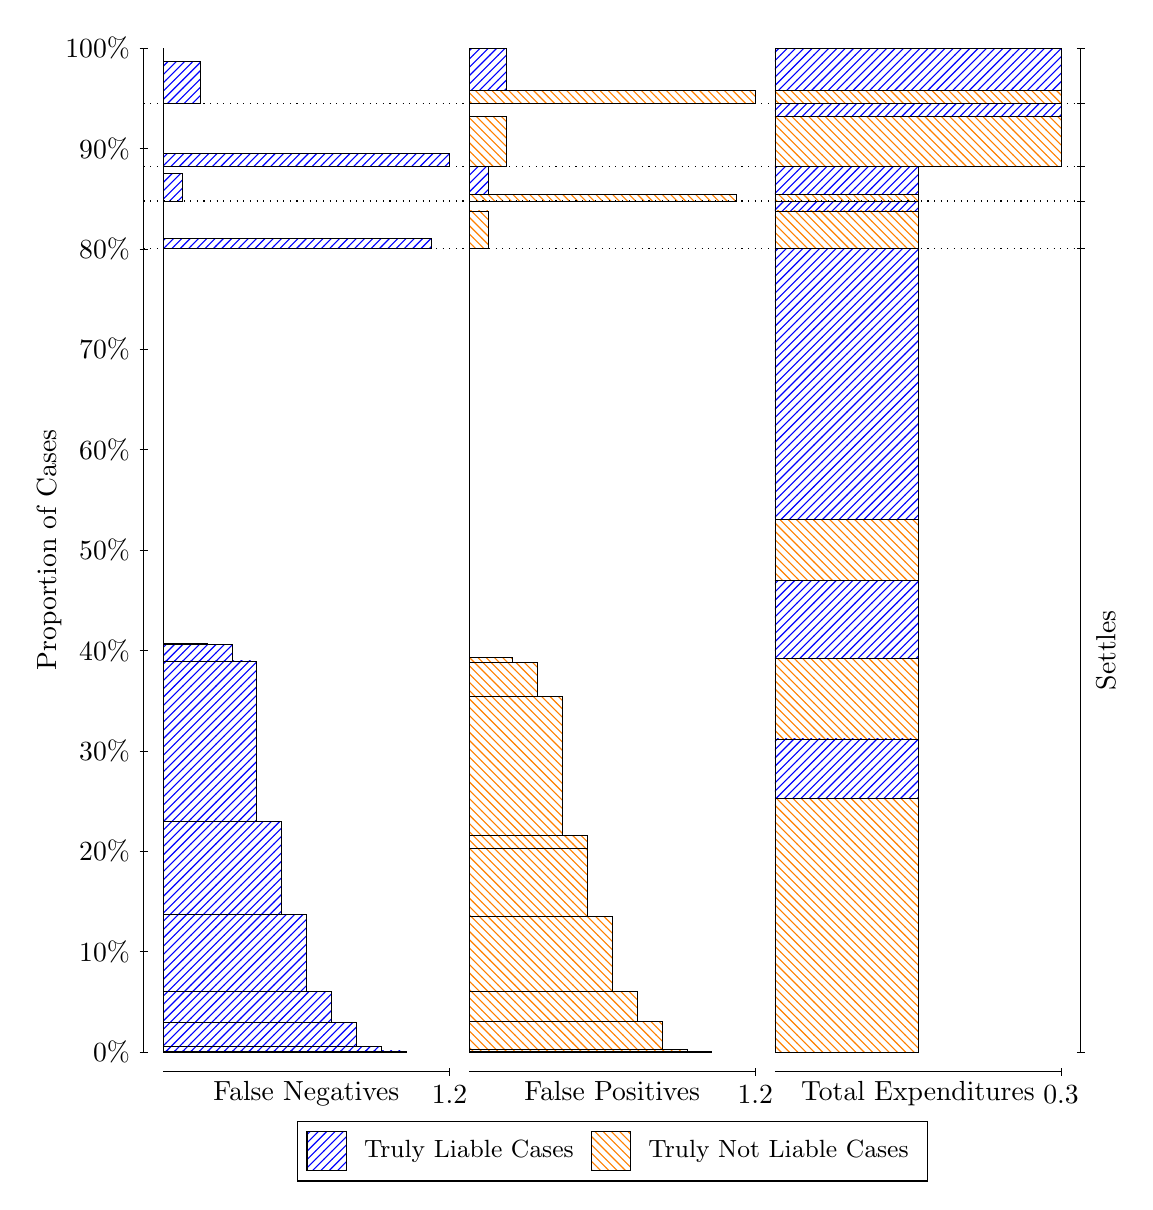
\begin{tikzpicture}
\draw[black, very thin] (1.5,1.75) -- (1.5,14.5);
\node[rotate=90, anchor=center] at (0.3, 8.125) {Proportion of Cases};
\draw[black, very thin] (1.45,1.75) -- (1.55,1.75);
\node[anchor=east] at (1.45, 1.75) {0\%};
\draw[black, very thin] (1.45,3.025) -- (1.55,3.025);
\node[anchor=east] at (1.45, 3.025) {10\%};
\draw[black, very thin] (1.45,4.3) -- (1.55,4.3);
\node[anchor=east] at (1.45, 4.3) {20\%};
\draw[black, very thin] (1.45,5.575) -- (1.55,5.575);
\node[anchor=east] at (1.45, 5.575) {30\%};
\draw[black, very thin] (1.45,6.85) -- (1.55,6.85);
\node[anchor=east] at (1.45, 6.85) {40\%};
\draw[black, very thin] (1.45,8.125) -- (1.55,8.125);
\node[anchor=east] at (1.45, 8.125) {50\%};
\draw[black, very thin] (1.45,9.4) -- (1.55,9.4);
\node[anchor=east] at (1.45, 9.4) {60\%};
\draw[black, very thin] (1.45,10.675) -- (1.55,10.675);
\node[anchor=east] at (1.45, 10.675) {70\%};
\draw[black, very thin] (1.45,11.95) -- (1.55,11.95);
\node[anchor=east] at (1.45, 11.95) {80\%};
\draw[black, very thin] (1.45,13.225) -- (1.55,13.225);
\node[anchor=east] at (1.45, 13.225) {90\%};
\draw[black, very thin] (1.45,14.5) -- (1.55,14.5);
\node[anchor=east] at (1.45, 14.5) {100\%};

\draw[black, very thin] (13.4,1.75) -- (13.4,14.5);
\draw[black, very thin] (13.35,1.75) -- (13.45,1.75);
\node[anchor=west] at (13.35, 1.75) {};
\draw[black, very thin] (13.35,11.954) -- (13.45,11.954);
\node[anchor=west] at (13.35, 11.954) {};
\draw[black, very thin] (13.35,12.557) -- (13.45,12.557);
\node[anchor=west] at (13.35, 12.557) {};
\draw[black, very thin] (13.35,12.994) -- (13.45,12.994);
\node[anchor=west] at (13.35, 12.994) {};
\draw[black, very thin] (13.35,13.795) -- (13.45,13.795);
\node[anchor=west] at (13.35, 13.795) {};
\draw[black, very thin] (13.35,14.5) -- (13.45,14.5);
\node[anchor=west] at (13.35, 14.5) {};

\draw[black, very thin, pattern color=blue, pattern=north east lines] (1.75,1.75) rectangle (4.8304,1.7627);
\draw[black, very thin, pattern color=blue, pattern=north east lines] (1.75,1.7627) rectangle (4.5145,1.8197);
\draw[black, very thin, pattern color=blue, pattern=north east lines] (1.75,1.8197) rectangle (4.1986,2.1276);
\draw[black, very thin, pattern color=blue, pattern=north east lines] (1.75,2.1276) rectangle (3.8826,2.5166);
\draw[black, very thin, pattern color=blue, pattern=north east lines] (1.75,2.5166) rectangle (3.5667,3.499);
\draw[black, very thin, pattern color=blue, pattern=north east lines] (1.75,3.499) rectangle (3.2507,4.679);
\draw[black, very thin, pattern color=blue, pattern=north east lines] (1.75,4.679) rectangle (2.9348,6.7155);
\draw[black, very thin, pattern color=blue, pattern=north east lines] (1.75,6.7155) rectangle (2.6188,6.9288);
\draw[black, very thin, pattern color=blue, pattern=north east lines] (1.75,6.9288) rectangle (2.3029,6.9415);
\draw[black, very thin, pattern color=orange, pattern=north west lines] (1.75,6.9415) rectangle (1.75,11.954);
\draw[black, very thin, pattern color=blue, pattern=north east lines] (1.75,11.954) rectangle (5.1464,12.08);
\draw[black, very thin, pattern color=orange, pattern=north west lines] (1.75,12.08) rectangle (1.75,12.557);
\draw[black, very thin, pattern color=blue, pattern=north east lines] (1.75,12.557) rectangle (1.987,12.909);
\draw[black, very thin, pattern color=orange, pattern=north west lines] (1.75,12.909) rectangle (1.75,12.994);
\draw[black, very thin, pattern color=blue, pattern=north east lines] (1.75,12.994) rectangle (5.3833,13.161);
\draw[black, very thin, pattern color=orange, pattern=north west lines] (1.75,13.161) rectangle (1.75,13.795);
\draw[black, very thin, pattern color=blue, pattern=north east lines] (1.75,13.795) rectangle (2.2239,14.334);
\draw[black, very thin, pattern color=orange, pattern=north west lines] (1.75,14.334) rectangle (1.75,14.5);
\draw[black, very thin, pattern color=orange, pattern=north west lines] (5.6333,1.75) rectangle (8.7138,1.756);
\draw[black, very thin, pattern color=orange, pattern=north west lines] (5.6333,1.756) rectangle (8.3978,1.7847);
\draw[black, very thin, pattern color=orange, pattern=north west lines] (5.6333,1.7847) rectangle (8.0819,2.1417);
\draw[black, very thin, pattern color=orange, pattern=north west lines] (5.6333,2.1417) rectangle (7.7659,2.5192);
\draw[black, very thin, pattern color=orange, pattern=north west lines] (5.6333,2.5192) rectangle (7.45,3.4756);
\draw[black, very thin, pattern color=orange, pattern=north west lines] (5.6333,3.4756) rectangle (7.1341,4.3308);
\draw[black, very thin, pattern color=orange, pattern=north west lines] (5.6333,4.3308) rectangle (7.1341,4.5029);
\draw[black, very thin, pattern color=orange, pattern=north west lines] (5.6333,4.5029) rectangle (6.8181,6.2646);
\draw[black, very thin, pattern color=orange, pattern=north west lines] (5.6333,6.2646) rectangle (6.5022,6.6973);
\draw[black, very thin, pattern color=orange, pattern=north west lines] (5.6333,6.6973) rectangle (6.1862,6.7627);
\draw[black, very thin, pattern color=blue, pattern=north east lines] (5.6333,6.7627) rectangle (5.6333,11.954);
\draw[black, very thin, pattern color=orange, pattern=north west lines] (5.6333,11.954) rectangle (5.8703,12.431);
\draw[black, very thin, pattern color=blue, pattern=north east lines] (5.6333,12.431) rectangle (5.6333,12.557);
\draw[black, very thin, pattern color=orange, pattern=north west lines] (5.6333,12.557) rectangle (9.0297,12.642);
\draw[black, very thin, pattern color=blue, pattern=north east lines] (5.6333,12.642) rectangle (5.8703,12.994);
\draw[black, very thin, pattern color=orange, pattern=north west lines] (5.6333,12.994) rectangle (6.1072,13.629);
\draw[black, very thin, pattern color=blue, pattern=north east lines] (5.6333,13.629) rectangle (5.6333,13.795);
\draw[black, very thin, pattern color=orange, pattern=north west lines] (5.6333,13.795) rectangle (9.2667,13.961);
\draw[black, very thin, pattern color=blue, pattern=north east lines] (5.6333,13.961) rectangle (6.1072,14.5);
\draw[black, very thin, pattern color=orange, pattern=north west lines] (9.5167,1.75) rectangle (11.333,4.9717);
\draw[black, very thin, pattern color=blue, pattern=north east lines] (9.5167,4.9717) rectangle (11.333,5.7255);
\draw[black, very thin, pattern color=orange, pattern=north west lines] (9.5167,5.7255) rectangle (11.333,6.7473);
\draw[black, very thin, pattern color=blue, pattern=north east lines] (9.5167,6.7473) rectangle (11.333,7.7425);
\draw[black, very thin, pattern color=orange, pattern=north west lines] (9.5167,7.7425) rectangle (11.333,8.5117);
\draw[black, very thin, pattern color=blue, pattern=north east lines] (9.5167,8.5117) rectangle (11.333,11.954);
\draw[black, very thin, pattern color=orange, pattern=north west lines] (9.5167,11.954) rectangle (11.333,12.431);
\draw[black, very thin, pattern color=blue, pattern=north east lines] (9.5167,12.431) rectangle (11.333,12.557);
\draw[black, very thin, pattern color=orange, pattern=north west lines] (9.5167,12.557) rectangle (11.333,12.642);
\draw[black, very thin, pattern color=blue, pattern=north east lines] (9.5167,12.642) rectangle (11.333,12.994);
\draw[black, very thin, pattern color=orange, pattern=north west lines] (9.5167,12.994) rectangle (13.15,13.629);
\draw[black, very thin, pattern color=blue, pattern=north east lines] (9.5167,13.629) rectangle (13.15,13.795);
\draw[black, very thin, pattern color=orange, pattern=north west lines] (9.5167,13.795) rectangle (13.15,13.961);
\draw[black, very thin, pattern color=blue, pattern=north east lines] (9.5167,13.961) rectangle (13.15,14.5);
\draw[black, dotted] (1.5,11.954) -- (13.4,11.954);
\draw[black, dotted] (1.5,12.557) -- (13.4,12.557);
\draw[black, dotted] (1.5,12.994) -- (13.4,12.994);
\draw[black, dotted] (1.5,13.795) -- (13.4,13.795);
\draw[black, very thin] (1.75,1.5) -- (5.3833,1.5);
\node[anchor=north] at (3.5667, 1.5) {False Negatives};
\draw[black, very thin] (5.3833,1.45) -- (5.3833,1.55);
\node[anchor=north] at (5.3833, 1.45) {1.2};

\draw[black, very thin] (5.6333,1.5) -- (9.2667,1.5);
\node[anchor=north] at (7.45, 1.5) {False Positives};
\draw[black, very thin] (9.2667,1.45) -- (9.2667,1.55);
\node[anchor=north] at (9.2667, 1.45) {1.2};

\draw[black, very thin] (9.5167,1.5) -- (13.15,1.5);
\node[anchor=north] at (11.333, 1.5) {Total Expenditures};
\draw[black, very thin] (13.15,1.45) -- (13.15,1.55);
\node[anchor=north] at (13.15, 1.45) {0.3};

\node[black, centered, rotate=90] at (13.72, 6.8521) {Settles};





\draw (7.449999999999999,1.5) node[draw=none] (baseCoordinate) {};
\begin{scope}[align=center]
        \matrix[scale=0.5, draw=black, below=0.5cm of baseCoordinate, nodes={draw}, column sep=0.1cm]{
            \node[rectangle, draw, minimum width=0.5cm, minimum height=0.5cm, pattern=north east lines, pattern color=blue] {}; &
            \node[draw=none, font=\small] (B) {Truly Liable Cases}; &
            \node[rectangle, draw, minimum width=0.5cm, minimum height=0.5cm, pattern=north west lines, pattern color=orange] {}; &
            \node[draw=none, font=\small] (B) {Truly Not Liable Cases}; \\
            };
\end{scope}

\end{tikzpicture}
\end{document}